\documentclass[12pt, a4paper]{report}
\usepackage{polyglossia}
\setdefaultlanguage{magyar}
\usepackage{mathtools}
\usepackage{amsthm}
\usepackage{fontspec}
\usepackage{unicode-math}
\setmainfont{GentiumPlus-R.ttf}[BoldFont=GenBasB.ttf,ItalicFont=GentiumPlus-I.ttf,BoldItalicFont=GenBasBI.ttf]
\setmathfont{TeX Gyre Pagella Math}
\defaultfontfeatures{Ligatures=TeX}
\usepackage[paper=a4paper,left=3.5cm,right=2.5cm,top=2.5cm,bottom=2.5cm]{geometry}
\usepackage{graphicx}
\usepackage{setspace}
\usepackage{indentfirst}
\usepackage[backend=biber,style=numeric,firstinits=true,sortlocale=hu,block=space,isbn=false,doi=false,url=false,maxbibnames=5]{biblatex}
\usepackage[style=english]{csquotes}
\addbibresource{bibliography.bib}
\usepackage[bookmarks,unicode,hyperfootnotes=false,pdfborder={0 0 0 0}]{hyperref}
\urlstyle{same}
\usepackage{titlesec}

\hypersetup{pdfauthor={Vadas Norbert},pdftitle={Élszínezések}}

\pagestyle{plain}
\onehalfspacing
\frenchspacing

\swapnumbers
\newtheorem{tét}{Tétel}[section]
\newtheorem{lem}[tét]{Lemma}
\newtheorem{áll}[tét]{Állítás}
\newtheorem{sej}[tét]{Sejtés}
\newtheorem{köv}[tét]{Következmény}
\theoremstyle{remark}
\newtheorem*{megj}{Megjegyzés}
\theoremstyle{definition}
\newtheorem{defi}{Definíció}[section]
\newtheorem{pl}{Példa}[section]

\DefineBibliographyStrings{english}{%
  and              = {és},
}

\makeatletter \renewcommand{\fnum@figure}{\thefigure.~\figurename} \makeatother

\begin{document}
\titleformat{\chapter}[hang]
    {\normalfont\LARGE\bfseries}{\thechapter.}{1em}{}

\begin{titlepage}
\begin{center}
{\huge \textsc{Eötvös Loránd Tudományegyetem \\ Természettudományi Kar \\}}
\hrulefill \\[2.5cm]
{\huge Vadas Norbert} \\[0.7cm]
{\Huge \textsc{Élszínezések}} \\[0.7cm]
alkalmazott matematikus MSc szakdolgozat \\[0.1cm]
operációkutatás szakirány \\[2.2cm]
{\large Témavezetõ:} \\[0.4cm]
{\Large Bérczi Kristóf} \\[0.3cm] 
{\Large Operációkutatási Tanszék}
\vfill

\includegraphics[width=0.3\textwidth]{./images/elte_cimer_szines} \\[0.5cm]
{\large Budapest, 2015}
\end{center}
\end{titlepage}

\pagenumbering{roman}
\tableofcontents

\chapter{Bevezetés} 
\pagenumbering{arabic}

\section{Fogalmak és jelölések}
A továbbiakban, hacsak nincs másképp jelezve, minden gráf egyszerű, véges és irányítatlan. Egy $G = (V, E)$ gráfon értelmezett $w: E \rightarrow [k] = \lbrace 1, \ldots, k \rbrace$ függvényt \textbf{$k$-élsúlyozás}nak nevezünk. Amennyiben a csúcsokhoz is rendelünk súlyokat, azaz $w: V \cup E \rightarrow [k]$, akkor \textbf{$k$-teljes-súlyozás}ról beszélünk. Egy csúcs \textbf{érték}én vagy \textbf{szín}én a rá illeszkedő élek súlyainak, és amennyiben van, a saját súlyának összegét értjük. Az első eset egy másik elnevezése még a \textbf{súlyozott fokszám}. Azt mondjuk, hogy egy súlyozás \textbf{csúcs-megkülönböztető}, ha bármely két csúcsnak különböző az értéke. Abban az esetben, ha ezt csak szomszédos csúcspárokra követeljük meg, akkor a csúcsok értékei egy helyes színezését adják a gráfnak. Az ilyen súlyozást \textbf{csúcs-színező}nek vagy \textbf{helyes}nek hívjuk. Adott $G$ gráfra a legkisebb olyan $k$ számot, melyre létezik $G$-nek csúcs-színező $k$-élsúlyozása, illetve $k$-teljes-súlyozása, rendre $\chi_e(G)$-vel, illetve $\chi_t(G)$-vel jelöljük. Végezetül egy gráfra azt mondjuk, hogy \textbf{rendes}, ha egyetlen komponense sem izomorf $K_2$-vel.

\section{Csúcsok színezése súlyozásokkal}
Az 1-2-3-sejtés vizsgálatát a gráfok irregularitásának vizsgálata motiválta. Egy gráf éleinek súlyozását irregulárisnak nevezzük, ha bármely két csúcsra a rájuk illeszkedő éleken vett összeg különböző. Egy gráf irregularitásának erősségén azt a legkisebb $k$ számot értjük, amelyre létezik irreguláris súlyozás az $\lbrace 1, \ldots, k \rbrace$ halmazból vett súlyokkal. Ennek a feladatnak egy természetesen adódó egyszerűsítése, ha csak szomszédos csúcsokra követeljük meg azt, hogy különböző legyen az értékük. 

A sejtést először \citeauthor{Karonski2004} \cite{Karonski2004} fogalmazta meg 2002-ben, és a következőképpen hangzik: 

\begin{sej}[Az 1-2-3-sejtés]
Minden rendes gráf élei megcímkézhetőek az 1, 2, 3 számokkal oly módon, hogy tetszőleges két szomszédos csúcsra a rájuk illeszkedő éleken lévő számok összege különböző legyen.
\end{sej}

A sejtést megfogalmazása óta sokat vizsgálták. Az eddigi legjobb korlátot \citeauthor{Kalkowski2010} \cite{Kalkowski2010} bizonyította be 2010-ben, mely szerint a helyes színezéshez öt élsúly elegendő. Világos, hogy $\chi_e(G) = 1$ pontosan akkor, ha a szomszédos csúcsok foka különböző. Könnyen látható az is, hogy léteznek olyan rendes gráfok, amelyekre nem elég két élsúly sem. Ilyen például a $3$ vagy $6$ hosszú kör. Így a legjobb remélhető általános korlát a $\chi_e(G) \leq 3$. Azonban egy aszimptotikus eredmény szerint egy $G(p, n)$ véletlen gráf majdnem biztosan megszínezhető csak az $1, 2$ élsúlyok segítségével \cite{AddarioBerry2008}. Bizonyos gráfosztályokra már sikerült igazolni a sejtést. Eszerint $3$-színezhető \cite{Karonski2004}, illetve teljes gráfok \cite{Alaeiyan2012} esetén $\chi_e(G) = 3$. Az előbbi eredmény nyomán feltehető az a kérdés, hogy mely páros gráfok esetében elegendő csak az $1, 2$ súlyok közül választani. \citeauthor{Lu2011} \cite{Lu2011} cikke szerint a $3$-összefüggő, valamint bizonyos fokszám-megkötéseknek eleget tevő páros gráfok ilyenek.

Hasonló sejtést fogalmazott meg teljes-súlyozásokra \citeauthor{Przybylo2010} 2008-ban:

\begin{sej}[Az 1-2-sejtés]
Minden gráf élei és csúcsai megcímkézhetőek az 1, 2 számokkal oly módon, hogy tetszőleges két szomszédos csúcsra a rájuk illeszkedő éleken és magán a csúcson lévő számok összege különböző legyen.
\end{sej}

Ebben a cikkben bebizonyították, hogy $\chi_t(G) \leq 11$, valamint $\chi_t(G) \leq \left( \left\lfloor \frac{χ(G)}{2} \right\rfloor + 1 \right)$. A jelenleg ismert legjobb eredmény szerint $\chi_t(G) \leq 3$.

A csúcs-színező élsúlyozásoknak számos változatát vizsgálták már az elmúlt évtizedben. Az irányított esetben egy digráf éleit súlyozzuk, a csúcsok értékét pedig csak a kifelé vezető éleken vett összeg határozza meg. Ez a probléma lényegesen egyszerűbb, mint az irányítatlan változat, ugyanis itt könnyedén belátható az 1-2-3-sejtéssel analóg állítás \cite{Baudon2014}.

\begin{áll}
Minden $D$ digráfra $\chi_e(D) = 3$.
\end{áll}

Más változatokban az élsúlyok összege helyett azok szorzata, halmaza, multihalmaza vagy sorozata határozza meg a csúcsok színeit. Emellett élsúlyozás helyett tekinthetünk csúcs-, illetve teljes-súlyozást is. Érdekes kérdés az is, hogy mit mondhatunk abban az esetben, ha a súlyokat nem az $\lbrace 1, \ldots, k \rbrace$ halmazból, hanem tetszőleges $k$-elemű listából választhatjuk ki. A különféle változatok eddigi eredményeiről \citeauthor{Seamone2012} \cite{Seamone2012} cikkében olvashatunk bővebben.

Természetesen adódik az a kérdés is, hogy vajon NP-nehéz-e annak eldöntése, hogy egy gráf színezéséhez 2 élsúly elegendő-e. A $\lbrace 0, 1 \rbrace$ és az $\lbrace 1, 2 \rbrace$ halmazok esetében, valamint irányított gráfokra a válasz igen, egyéb esetben ez egy nyitott probléma.

\chapter{Élsúlyozások és az 1-2-3-sejtés}
A sejtéssel kapcsolatban a legfontosabb előrehaladást tetszőleges $G$ gráf esetén a $\chi_e(G)$-re vonatkozó konstans korlátok bevezetése és javítása jelenti. A sejtést először felvető cikkben még csak azt bizonyították, hogy véges sok valós élsúly elegendő, később viszont egész számokra vonatkozó korlátokat is adtak. A jelenleg ismert legjobb eredmény \citeauthor{Kalkowski2010} nevéhez fűződik, akik a $\chi_e(G) \leq 6$ \cite{Kalkowski2009}, kicsivel később pedig a $\chi_e(G) \leq 5$ \cite{Kalkowski2010} korlátot adták a problémára. A két bizonyítás merőben más eszközöket használ, amelyek önmagukban is említésre érdemesek, ezért a következőkben mindkettőre kitérünk.

\section{Csúcs-színező 6-élsúlyozás}
Először vizsgáljuk a gyengébb korlátot. Az erre vonatkozó tétel bizonyítása előtt tekintsük a következő lemmát, mely az \cite{Kalkowski2009} cikk első szerzőjének egy korábbi eredménye:

\begin{lem}
Minden összefüggő, rendes $G$ gráfra létezik olyan $f:E(G) \rightarrow \lbrace 1, 2, 3 \rbrace$ élsúlyozás és $f':V(G) \rightarrow \lbrace 0, 1 \rbrace$ csúcs-súlyozás, melyre a csúcsok $w(v) = f'(v) + \sum\limits_{w \in N(v)} f(vw)$ értéke egy helyes színezés.
\end{lem}

Ennek segítségével egy $\chi_e(G) \leq 10$ korlát adható az élsúlyok megháromszorozásával, majd bizonyos élek $1$-gyel történő módosításával. Jelen esetben is egy hasonló eljárást követünk majd, amelyhez szükségünk lesz a lemma egy általánosabb alakjára. Előtte azonban érdemes megjegyezni egy egyszerű következményt. A sejtés vizsgálatánál érdekes kérdés lehet, hogy mit tudunk mondani a rossz élek részgráfjáról, vagyis azon élekről, melyek végpontjai azonos értékűek. A fenti lemma erre is ad egyfajta választ, ugyanis az általa biztosított teljes-súlyozásban minden csúcsra $0$-t írva olyan élsúlyozást kapunk, ahol a rossz élek egy páros gráfot alkotnak. Ez a megfigyelés segíthet abban, hogy közelebb jussunk a sejtés bizonyításához vagy cáfolatához. Visszatérve a tételünkhöz, a lemma általánosítása a következőképpen hangzik:

\begin{lem} \label{lem:edge6treemixed}
Legyen $\alpha \in \mathbb{R}$ és $\beta \in \mathbb{R} \smallsetminus \lbrace 0 \rbrace$. Ekkor minden összefüggő, rendes $G$ gráfra, és tetszőleges $T$ feszítőfájára létezik olyan $f:E(G) \rightarrow \lbrace \alpha - \beta, \alpha, \alpha + \beta \rbrace$ élsúlyozás és $f':V(G) \rightarrow \lbrace 0, \beta \rbrace$ csúcs-súlyozás, melyre a csúcsok $w(v) = f'(v) + \sum\limits_{w \in N(v)} f(vw)$ értéke egy helyes színezés. Továbbá $f$ megválasztható úgy, hogy $f(e) = \alpha$ minden $e \in E(T)$-re.
\end{lem}

\begin{proof}
Legyen $v_1, v_2, \ldots, v_n$ a csúcsoknak egy olyan sorrendje, melyre minden $k \geq 2$-re $v_k$-ból pontosan egy $T$-beli él vezet $\lbrace v_1, v_2, \ldots, v_{k - 1} \rbrace$-be. Kezdetben minden élhez az $\alpha$ súlyt rendeljük, amelyet legfeljebb egyszer módosítunk, hogy sorban minden $v_k$ csúcs értékét véglegesítsük.

Legyen $w(v_1) = \alpha d(v_1)$, és tegyük fel, hogy valamely $k \geq 2$-re már meghatároztuk az $f$ élsúlyokat az $E(G\lbrack \lbrace v_1, v_2, \ldots, v_{k - 1} \rbrace \rbrack) \smallsetminus E(T)$ halmazon és az $f'$ csúcs-súlyokat $\lbrace v_1, v_2, \ldots, v_{k - 1} \rbrace$-en úgy, hogy az első $k - 1$ csúcs $w(v_i)$ értéke már végleges.

A $v_k$ csúcs esetén minden $E(v_k, \lbrace v_1, v_2, \ldots, v_{k - 1} \rbrace) \smallsetminus E(T)$-beli él súlyát módosíthatjuk $\beta$-val. Amennyiben $v_k v_i \in E(G) \smallsetminus E(T)$ és $f'(v_i) = 0$, akkor választhatunk $(f(v_k v_i) = \alpha, f'(v_i) = 0)$ és $(f(v_k v_i) = \alpha - \beta, f'(v_i) = \beta)$ között anélkül, hogy megváltoztatnánk $w(v_i)$-t. Hasonlóan, ha $v_k v_i \in E(G) \smallsetminus E(T)$ és $f'(v_i) = \beta$, akkor választhatunk $(f(v_k v_i) = \alpha, f'(v_i) = \beta)$ és $(f(v_k v_i) = \alpha + \beta, f'(v_i) = 0)$ között anélkül, hogy megváltoztatnánk $w(v_i)$-t. Végezetül megválaszthatjuk $f'(v_k)$ értékét is. Ez összesen $|E(v_k, \lbrace v_1, v_2, \ldots, v_{k - 1} \rbrace) \smallsetminus E(T)| + 2 = |E(v_k, \lbrace v_1, v_2, \ldots, v_{k - 1} \rbrace)| + 1$ különböző lehetőség $w(v_k)$ értékének, melyek közül kiválaszthatjuk azt, amely minden $N(v_k) \cap \lbrace v_1, v_2, \ldots, v_{k - 1} \rbrace$-beli csúcs értékétől különbözik.

Ezt az eljárást folytatva megkaphatjuk a kívánt súlyozást.
\end{proof}

Ezen lemma birtokában most már készen állunk a tétel bizonyítására.

\begin{tét}[\citeauthor{Kalkowski2009} \cite{Kalkowski2009}]
Minden $G$ rendes gráfra $\chi_e(G) \leq 6$.
\end{tét}

\begin{proof}
Feltehető, hogy $G$ összefüggő, különben a komponenseket külön-külön vizsgálhatjuk. Induljunk ki egy tetszőleges $T$ feszítőfából, és vegyünk egy $(f, f', w)$ súlyozást a lemma alapján, $\alpha = 4$ és $\beta = -2$ paraméterekkel. Ekkor minden csúcs és él súlya páros. A bizonyítás hátralévő részében módosítani fogjuk $f$-et és $f'$-t, de $w(v)$ változatlan marad minden $v \in V(G)$ csúcsra.

Legyen $H = G\lbrack \lbrace v \in v(G)\ |\ f'(v) = -2 \rbrace \rbrack$, és ebben $H_1$ egy maximális feszítő részgráf, melyben a legnagyobb fokszám legfeljebb $2$. Adjunk hozzá $-1$-et $f(e)$-hez a $H_1$ minden $e$ élére, és módosítsuk $V(H_1)$ minden $v$ csúcsán az $f'(v)$ értéket ennek megfelelően, hogy $w(v)$ változatlan maradjon. Így minden $v \in V(G)$ csúcsra $f'(V) \in \lbrace 0, -1, -2 \rbrace$, minden $e \in E(G)$ élre $f(e) \in \lbrace 1, 2, \ldots, 6 \rbrace$, továbbá minden $e \in E(T)$ élre $f(e) \in \lbrace 3, 4 \rbrace$.

Legyen $i \in \lbrace 0, 1, 2 \rbrace$ esetén $S_i = \lbrace v \in v(G)\ |\ f'(v) = -i \rbrace$ és $s_i = |S_i|$. Figyeljük meg, hogy minden $v \in S_0 \cup S_2$ csúcs $w(v) - f'(v)$ súlya páros, az $S_1$-beli csúcsoké pedig páratlan. $H_1$ maximalitása miatt minden $uv$ élre, ahol $u, v \in S_1 \cup S_2$, teljesül, hogy $u, v \in S_1$ és $uv \in E(H_1)$, hiszen ha nem így lenne, akkor az előző lépésben a $H_1$ részgráfot tudtuk volna még bővíteni. Részletesebben, ezen élek végpontjaira $w(u) - f'(u) \neq w(v) - f'(v)$. Az ilyen élek halmazát jelölje $E^*$.

Ha $s_2 = 0$, akkor készen vagyunk, hiszen $f$ jó színezést ad. Amennyiben $s_2 = 1$ és $s_1 = 0$, legyen $u \in S_2$. Figyeljük meg, hogy minden $u$-ra illeszkedő $e$ él súlya $f(e) \in \lbrace 2, 4, 6 \rbrace$. Ha $u$-nak van egy olyan $v$ szomszédja, melyre $w(u) + 2 \neq w(v)$, akkor az $uv$ és súlyát $1$-gyel csökkentve szintén helyes színezéshez jutunk. (Figyeljük meg, hogy csak $u$ és $v$ súlya páratlan.) Ha $u$ minden $v \in N(u)$ szomszédjára $w(u) + 2 = w(v)$ és $|N(u)| \geq 2$, akkor két különböző, $u$-ra illeszkedő élen is csökkentsük a súlyt $1$-gyel. Ez ismét a kívánt súlyozáshoz vezet. Végül, ha az $u$ csúcs egyetlen $v$ szomszédjára $w(u) + 2 = w(v)$, akkor vegyünk egy $x \in N_T(v) \smallsetminus \lbrace u \rbrace$ csúcsot, csökkentsük $f(uv)$-t $1$-gyel, $f(vx)$-et pedig növeljük $1$-gyel. Így ismét megfelelő súlyozást kapunk.

Ha $s_2 = 1$ és $s_1 \geq 1$, akkor vegyünk egy $T$-beli utat $u \in S_2$ és egy $v \in S_1$ között, majd felváltva csökkentsük és növeljük az élek súlyát $1$-gyel, ügyelve arra, hogy a $v$-re illeszkedő él súlyát csökkentsük. Ezzel a keresett súlyozáshoz jutunk.

Ha $s_2 \geq 2$, akkor indukcióval beláthatjuk, hogy tudunk találni $\left\lceil \frac{s_2}{2} \right\rceil$ olyan $T$-beli utat, melyek végpontjai pontosan az $S_2$-beli csúcsok, és amelyek $T$ minden élét legfeljebb kétszer használják. Ilyen utakat $2 \leq s_2 \leq 3$ esetén könnyen találhatunk. Amennyiben $s_2 \geq 4$, úgy keressünk egy olyan $e \in E(T)$ élt, melyre $T-e$ mindkét komponense legalább $2$ $S_2$-beli csúcsot tartalmaz, és legalább az egyikben páros számú ilyen csúcs van. A két komponensre indukciót alkalmazva megtalálhatjuk a keresett utakat.

Felváltva csökkentsük és növeljük ezen utak mentén az élek súlyait úgy, hogy csak a végpontok súlya változzon, és módosítsuk ennek megfelelően az $f'$ értékeket ezeken a csúcsokon. Ha egy $u \in S_2$ csúcs két útnak is végpontja (például, ha $s_2$ páratlan), akkor ügyeljünk arra, hogy az $u$-ra illeszkedő mindkét élen csökkentsük a súlyt, hogy $f'(u) = 0$ adódjon. Figyeljük meg, hogy csak $E(T)$-beli éleket használunk, így nem kapunk $1$-nél kisebb vagy $6$-nál nagyobb élsúlyokat. Ezek után minden csúcsra, amely korábban $S_2$-ben volt, $f'(v) \in \lbrace -3, -1, 0 \rbrace$. Könnyen látható, hogy így az $f$ súlyozást tekintve minden $v$ csúcs értéke $w(v)$, amennyiben $w(v)$ páros. A páratlan értékű csúcsok között futó élek mind $E^*$-ban vannak, tehát a végpontjaik $w$ súlya különböző, ahogyan azt korábban már láttuk. Így $f$ egy csúcs-színező $6$-élsúlyozás.
\end{proof}

\section{Csúcs-színező 5-élsúlyozás}
\begin{tét}[\citeauthor{Kalkowski2010} \cite{Kalkowski2010}]
Minden $G$ rendes gráfra $\chi_e(G) \leq 5$.
\end{tét}

\begin{proof}
Feltehető, hogy $G$ összefüggő, különben komponensenként érvelhetünk. Feltehető még továbbá az is, hogy $|V| \geq 3$, és létezik olyan $v$ csúcs, melyre $d(v) \geq 2$. Legyen $v_1, v_2, \ldots, v_n$ a csúcsoknak egy olyan sorrendje, melyre $d(v_n) \geq 2$, és minden $1 \leq i \leq n-1$-re $v_i$-nek van szomszédja $\lbrace v_{i+1}, v_{i+2}, \ldots, v_n \rbrace$-ben.

Kezdetben minden $e$ élhez az $f(e) = 3$ élsúlyt rendeljük, majd legfeljebb kétszer módosítjuk, miközben sorban végighaladunk a csúcsokon. Minden $i < n$-re a $v_i$ csúcshoz hozzárendelünk két színt, $W(v_i) = \lbrace w(v_i), w(v_i) +2 \rbrace$, ahol $w(v_i) \in \lbrace 0, 1 \rbrace$ mod $4$, oly módon, hogy minden $v_j v_i \in E$ élre, ahol $1 \leq j < i$, $W(v_j) \cap W(v_i) = \emptyset$, és biztosítani fogjuk, hogy $f(v_i) = \sum\limits_{u \in N(v_i)} f(uv_i) \in W(v_i)$. Végül beállítjuk a $v_n$-re illeszkedő élek súlyát úgy, hogy $f(v_n)$ különbözzön $f(v_i)$-től minden $v_i \in N(v_n)$-re.

Ezt szem előtt tartva legyen $f(v_1) = 3d(v_1)$, és válasszuk meg a $W(v_1)$ halmazt úgy, hogy $f(v_1) \in W(v_1)$, valamint $w(v_1) \in \lbrace 0, 1 \rbrace$ mod $4$ teljesüljön. Legyen $2 \leq k \leq n - 1$, és tegyük fel, hogy már minden $i < k$-ra meghatároztuk $W(v_i)$-t, valamint
\begin{itemize}
\item $f(v_i) \in W(v_i)$, ahol $i < k$
\item $f(v_k v_j) = 3$ minden élre, ahol $j > k$
\item ha $f(v_i v_k) \neq 3$ valamely élre $i < k$ esetén, akkor vagy $f(v_i v_k) = 2$ és $f(v_i) = w(v_i)$, vagy $f(v_i v_k) = 4$ és $f(v_i) = w(v_i) + 2$.
\end{itemize}

Ha $v_i v_k \in E$ valamely $i < k$-ra, akkor $f(v_i v_k)$-t $2$-vel növelhetjük vagy csökkenthetjük úgy, hogy $f(v_i) \in W(v_i)$ maradjon. Amennyiben $v_k$-nak $d$ ilyen szomszédja van, úgy ez $d + 1$ lehetséges értéket jelent $f(v_k)$ számára, melyek mind azonos paritásúak. Ezen felül megengedjük még, hogy az $f(v_k v_j)$ súlyt $1$-gyel módosítsuk, ahol $j > k$ a legkisebb index, melyre $v_k v_j \in E$. Ezáltal $f(v_k)$ egy $\lbrack a, a + 2d + 2 \rbrack$ intervallum minden értékét felveheti. Úgy szeretnénk módosítani a súlyokat és meghatározni $w(v_k)$-t, hogy
\begin{enumerate}
\item $f(v_i) \in W(v_i)$, ahol $1 \leq i \leq k$
\item $v_i v_k \in E$ esetén $w(v_i) \neq w(v_k)$, ahol $i < k$
\item vagy $f(v_k) = w(v_k)$ és $f(v_k v_j) \in \lbrace 2, 3 \rbrace$ vagy $f(v_k) = w(v_k) + 2$ és $f(v_k v_j) \in \lbrace 3, 4 \rbrace$
\end{enumerate}
teljesüljön. A második feltétel legfeljebb $2d$ értéket zárhat ki az $\lbrack a, a + 2d + 2 \rbrack$ intervallumból, míg a harmadik feltétel csak az $a$ és $a + 2d + 2$ értékeket, hiszen minden más $f(v_k)$ értékre $f(v_k v_j) \neq 3$ esetén lehetőségünk van választani $f(v_k v_j) = 2$ és $f(v_k v_j) = 4$ között. Így legalább egy érték szabadon marad $f(v_k)$ számára.

Ilyen módon lépésről lépésre, konfliktus nélkül meghatározhatjuk a $W(v_k)$ halmazokat minden $k \leq n - 1$-re. Vegyük észre, hogy amikor az $f(v_k)$ érték először változik meg egy $v_k v_i$, $i > k$ él módosítása miatt, akkor $i = j$, vagyis nem okoznak problémát a $2$ vagy $4$ súlyú élek.

Utolsó lépésként találnunk kell egy szabad értéket $v_n$-nek. Ez alkalommal nem áll rendelkezésünkre egy $v_n v_j$ segédél, de nem is kell későbbi csúcsok miatt aggódnunk. Az előzőekhez hasonlóan, ha $v_i v_n \in E$ valamely $i < n$-re, akkor $f(v_i v_n)$-t $2$-vel növelhetjük vagy csökkenthetjük úgy, hogy $f(v_i) \in W(v_i)$ maradjon. Ezek a módosítások összesen $d(v_n) +1 \geq 3$, azonos paritású lehetőséget jelentenek $f(v_n)$ értékének. Így, ha a legkisebb ilyen lehetséges $a$ értékre $a \in \lbrace 2, 3 \rbrace\ \mathrm{mod}\ 4$, akkor minden $v_n$-re illeszkedő élen a kisebb értéket választva a csúcsok egy helyes színezését kapjuk. Ha $a \in \lbrace 0, 1 \rbrace\ \mathrm{mod}\ 4$, és létezik olyan $v_i \in N(v_n)$ csúcs, melyre $w(v_i) \neq a$, akkor a $v_i v_n$ élen a nagyobb, minden más élen pedig a kisebb súlyt választva $f(v_n) = a + 2$, ami szintén helyes színezéshez vezet. Végezetül, amennyiben $a \in \lbrace 0, 1 \rbrace\ \mathrm{mod}\ 4$ és $w(v_i) = a$ minden $v_i \in N(v_n)$-re, akkor legalább két élen a nagyobb súlyt választva kapunk helyes színezést. Ezzel a tétel állítását beláttuk.
\end{proof}

\section{Csúcs-színező 3-élsúlyozás irányított gráfokra}
Az eddigiekben irányítatlan gráfok élsúlyozásait vizsgáltuk, de joggal merülhet fel a kérdés, hogy vajon mit tudunk mondani az irányított esetről. Itt két lehetőségünk van egy csúcs színének meghatározására. 

Az első esetben a kimenő élek összsúlyából kivonjuk bemenő élek összsúlyát. Erről a változatról \citeauthor{Bartnicki2009} \cite{Bartnicki2009} bebizonyították, hogy a súlyokat tetszőleges kételemű listákról választva is létezik csúcs-színező élsúlyozás.

A második esetben egy csúcs színét csak a kimenő éleken vett súlyok összege, azaz a csúcs súlyozott kifoka határozza meg. A továbbiakban ezzel az esettel fogunk foglalkozni.

Könnyen látható, hogy léteznek olyan digráfok, például a $3$ hosszú irányított kör, amelyek helyes színezéséhez nem elegendőek az $\lbrace 1, 2 \rbrace$ élsúlyok. A következő tétel azt mondja ki, hogy minden irányított gráfnak van csúcs-színező 3-élsúlyozása. Ez abból következik, hogy minden digráfnak van egy alkalmas csúcsa, amely a szomszédai számához képest sok lehetséges súlyozott kifok-értéket vehet fel. Egy ilyen csúcs létezése teljes indukció használatát teszi lehetővé, továbbá a bizonyítás polinomiális idejű algoritmust is eredményez egy csúcs-színező 3-élsúlyozás megtalálására.

\begin{tét}[\citeauthor{Baudon2014} \cite{Baudon2014}]
Minden $D$ digráfra $\chi_e(D) \leq 3$.
\end{tét}

\begin{proof}
A bizonyítás $D$ élszáma szerinti indukcióval történik. Az állítás nyilvánvaló $0$ vagy $1$ élű digráf esetén. Tegyük fel, hogy legfeljebb $m - 1$ élre már igazoltuk a tételt, és legyen $D = (V, A)$ egy $m \geq 2$ élű digráf.

Figyeljük meg, hogy $D$-nek létezik egy olyan $v$ csúcsa, melyre $\delta(v) > 0$ és $\delta(v) > \varrho(v)$, hiszen különben $\sum\limits_{v \in V} \varrho(v) \neq \sum\limits_{v \in V} \delta(v)$ lenne. Első lépésként töröljünk minden $v$-ből kilépő élet. Ekkor az indukciós feltevés miatt a fennmaradó digráfnak létezik egy $w$ csúcs-színező 3-élsúlyozása. Tegyük vissza a kitörölt éleket, és terjesszük ki ezekre $w$-t oly módon, hogy $v$ súlyozott kifoka különbözzön mind a $\delta(v) + \varrho(v)$ szomszédjáétól. Ez megtehető, hiszen $2\delta(v) + 1$ érték közül választhatunk, nevezetesen a $\lbrace \delta(v), \delta(v) + 1, \ldots, 3\delta(v) \rbrace$ halmazból, míg a tiltott értékek száma $v$ választása miatt legfeljebb $\varrho(v) + \delta(v) < 2\delta(v) + 1$. Mivel ezen élsúlyok kizárólag a $v$ csúcs súlyozott kifokát befolyásolják, ezért az így kapott kiterjesztett súlyozás a $D$ digráf egy csúcs-színező 3-élsúlyozása.
\end{proof}

Ebben a bizonyításban azt használtuk ki, hogy egy $d$-edfokú csúcs lehetséges súlyozott kifokainak száma kellően nagy, pontosabban legalább $2d + 1$, amennyiben az éleket az $\lbrace 1, 2, 3 \rbrace$ számokkal súlyozzuk. Most megmutatjuk, hogy ez a tulajdonság tetszőleges $\lbrace a, b, c \rbrace$ súlyok esetén fennáll, és így egy erősebb tétel is igaz.

\begin{lem}
Legyen egy $D$ digráfnak $v$ egy legalább $d$-edfokú csúcsa, valamint $a, b$ és $c$ három valós szám. Ekkor $v$ súlyozott kifoka legalább $2d + 1$ különböző értéket vehet fel $D$ egy tetszőleges élsúlyozásában, amelyben a $v$-ből kimenő élek súlyai az $\lbrace a, b, c \rbrace$ halmazból kerülnek ki.
\end{lem}

\begin{proof}
A bizonyítás $d$ szerinti indukcióval történik. Amennyiben $d = 1$, úgy a $v$-ből kilépő él súlya $a, b$ vagy $c$ lehet. Mivel ezek különbözőek, ezért $v$ súlyozott kifokának is $3$ különböző értéke lehet.

Tegyük fel, hogy $d \leq i - 1$ esetén már igazoltuk az állítást, és legyen $d = i$. Jelölje $D'$ azt a digráfot, amelyet egy $v$-ből kilépő $vu$ él elhagyásával kapunk $D$-ből. Ekkor az indukciós feltevés szerint $v$ súlyozott kifoka legalább $2(d - 1) + 1$ lehetséges értéket vehet fel $D$ egy tetszőleges élsúlyozásában, amely a $v$-ből kilépő éleket az $\lbrace a, b, c \rbrace$ számokkal súlyozza. Legyen $F'$ ezen lehetséges értékek halmaza, valamint $k$ és $n$ rendre a legkisebb, illetve legnagyobb eleme $F'$-nek, továbbá $w_K$ és $w_N$ két élsúlyozása $D'$-nek, melyekre a $v$ csúcs súlyozott kifoka rendre $K$, illetve $N$.

Tegyük fel, hogy $a < b < c$. Amennyiben az állítás igaz az $\lbrace a, b, c \rbrace$ számokra, úgy igaz a $\lbrace -a, -b, -c \rbrace$ számokra is, ezért két eset lehetséges:

\begin{enumerate}
\item $0 \leq a < b < c$
\item $a < 0 \leq b < c$
\end{enumerate}

Az első esetben terjesszük ki a $D'$ minden élsúlyozását a $D$ digráfra úgy, hogy a $vu$ élre $a$ súlyt írunk. Ekkor azt kapjuk, hogy az $F = \lbrace x + a: x \in F' \rbrace$ halmaz a $v$ csúcs lehetséges súlyozott kifokainak $2(d - 1) + 1$ elemű halmaza. A fennmaradó két lehetőséget úgy kapjuk, hogy a $w_N$ súlyozást $b$ vagy $c$ értékkel kiterjesztjük a $vu$ élre. Ekkor ugyanis $N + b$ és $N + c$ két újabb lehetséges érték, hiszen $a < b < c$ miatt ezek nincsenek $F$-ben. Tehát létezik legalább $2d + 1$ választás $v$ súlyozott kifokára.

A második esetben terjesszük ki a $D'$ minden élsúlyozását a $D$ digráfra úgy, hogy a $vu$ élre $b$ súlyt írunk. Ekkor azt kapjuk, hogy az $F = \lbrace x + b: x \in F' \rbrace$ halmaz a $v$ csúcs lehetséges súlyozott kifokainak $2(d - 1) + 1$ elemű halmaza. A fennmaradó két lehetőséget úgy kapjuk, hogy a $w_N$ és $w_K$ súlyozásokat rendre $a$, illetve $c$ értékkel kiterjesztjük a $vu$ élre. Ezekből azt kapjuk, hogy $K + a$ és $N + c$ két újabb lehetséges érték, amely nem szerepel $F$-ben a súlyokra vonatkozó feltevés miatt. Ezzel az állítást beláttuk.
\end{proof}

A lemma következményeként azt kapjuk, hogy az előző tétel bizonyításában nem számít, hogy egy csúcsnál mely három súlyt írhatjuk a kimenő élekre. Ez a megfigyelés az alábbi listaszínezési tételhez vezet.

\begin{tét}
Legyen adott egy $D$ digráf minden $v$ csúcsára egy három valós számból álló $L(v)$ lista. Ekkor $D$-nek van olyan csúcs-színező élsúlyozása, amelyben minden $v$ csúcsra a kimenő élek súlyai $L(v)$-ből kerülnek ki.
\end{tét}

A probléma egyfajta kiterjesztéseként megkérdezhetjük, hogy melyik az a legkisebb $k \in \lbrace 1, 2, 3 \rbrace$, melyre minden irányított gráfnak létezik olyan irányítása, amelynek van csúcs-színező $k$-élsúlyozása. Tudjuk, hogy egy digráfnak pontosan akkor létezik csúcs-színező $1$-élsúlyozása, ha bármely két szomszédos pont kifoka különböző. A következő lemma azt mondja ki, hogy minden gráfnak létezik olyan irányítása, amelyre ez teljesül.

\begin{lem}
Minden $G$ gráfnak létezik olyan irányítása, amelyben bármely két szomszédos csúcs kifoka különböző.
\end{lem}

\begin{proof}
A bizonyítás $G$ pontszáma szerinti indukcióval történik. Az állítás $n \leq 2$ esetén nyilvánvaló. Tegyük fel, hogy legfeljebb $i - 1$ csúcsra már igaz a lemma, és legyen $G$ egy $n = i$ pontú gráf. Jelölje $v$ a legnagyobb fokszámú csúcsot $G$-ben. Az indukciós feltevés szerint $G' = G - v$ megirányítható úgy, hogy bármely két szomszédos csúcs kifoka különböző legyen. Jelölje az így kapott digráfot $D'$. Figyeljük meg, hogy $v$ választása miatt $D'$-ben minden $v$-vel szomszédos csúcs kifoka legfeljebb $d(v) - 1$. Legyen $D$ a $G$ gráf azon irányítása, amelyet a $D'$ irányításból kapunk oly módon, hogy a $v$-re illeszkedő éleket mind kifelé irányítjuk. Mivel így $v$ kifoka a $D$ digráfban $d(v)$, és a szomszédos csúcsok kifoka nem változott, ezért a kapott irányítás továbbra is teljesíti a lemma feltételét.
\end{proof}

Ezen lemma ismeretében és a korábbi megfigyelésünk alapján az alábbi tételt fogalmazhatjuk meg:

\begin{tét}
Minden irányítatlan gráfnak létezik olyan irányítása, amelynek van csúcs-színező $1$-élsúlyozása.
\end{tét}

\chapter{Teljes súlyozások és az 1-2-sejtés}

\section{Csúcs-színező $\left( \left\lfloor \frac{χ(G)}{2} \right\rfloor + 1 \right)$-tejes-súlyozás}

\begin{áll}
Minden $G$ páros gráfra $\chi_t(G) \leq 2$.
\end{áll}

\begin{proof}
Rendeljük a gráf éleihez az $1, 2$ súlyokat tetszőleges módon. Ezután válasszuk meg a csúcsok súlyát úgy, hogy az egyik színosztályban minden csúcs összsúlya páros, a másik színosztályban pedig páratlan legyen.
\end{proof}

Hasonló gondolatmenettel kapjuk az alábbi, általánosabb megfigyelésünket is:

\begin{áll}
Legyen adott a $G$ gráf és minden $v \in V(G)$ csúcsra egy $t_v$ szín. Ekkor $G$-nek létezik olyan $2$-tejes-súlyozása, hogy $c(v) ≡ t_v\ (\mathrm{mod}\ 2)$ minden $v \in V(G)$-re. 
\end{áll}

A következőkben egy még általánosabb állítást fogunk igazolni, amelynek segítségével felülről tudjuk majd becsülni $\chi_t(G)$-t a $G$ kromatikus számával.

\begin{lem} \label{lem:totalcircle}
Legyen adott egy $C$ kör, minden $v \in V(C)$ csúcsra egy $t_v$ szín, és $p \geq 3$ egész. Ekkor $C$-nek létezik olyan $\left( \left\lfloor \frac{p}{2} \right\rfloor + 1 \right)$-tejes-súlyozása, hogy $c(v) ≡ t_v\ (\mathrm{mod}\ p)$ minden $v \in V(C)$-re.
\end{lem}

\begin{proof}
Legyenek $C$ csúcsai sorban $v_1, v_2, \ldots, v_n$, ahol $n = |C|$. Feltehetjük, hogy minden $i$-re $t_{v_i} \in \lbrack 3, p + 2 \rbrack$. Legyen $V(C) = S \cup L$, ahol $v_i \in S$, ha $t_{v_i} \in \lbrack 3, \left\lfloor \frac{p}{2} \right\rfloor + 2 \rbrack$, valamint $v_i \in L$, ha $t_{v_i} \in \lbrack \left\lfloor \frac{p}{2} \right\rfloor + 3, p + 2 \rbrack$. Jelölje a $t_{v_i}$ színt $s_i$, ha $v_i \in S$, illetve $l_i$, ha $v_i \in L$, és legyen $h = \left\lfloor \frac{p}{2} \right\rfloor + 1$. A továbbiakban csak az $1, 2, \ldots, h$ súlyokat fogjuk használni. 

Először is figyeljük meg, hogy ha $|L|$ páros, akkor könnyedén megkaphatjuk a kívánt súlyozást. Ehhez elég csak az $1, h$ súlyokat használni az éleken. Kezdetnek legyen $w(v_n v_1) = 1$, és ezután sorban rendeljük hozzá az $1, h$ súlyokat az élekhez oly módon, hogy a $v_i$-re illeszkedő két él súlya azonos legyen, ha $v_i \in S$, illetve különböző, ha $v_i \in L$. Így a jelenlegi összsúlyok értéke $\mathrm{mod}\ p$ az $S$-beli csúcsok esetén $1$ vagy $2$ ($p$ paritásától függően), illetve $\left\lfloor \frac{p}{2} \right\rfloor + 2$ az $L$-beli csúcsokra. Innen már könnyedén befejezhető a súlyozás a csúcsok súlyainak megválasztásával.

Legyen $|L|$ páratlan, és legyen $v_2 \in L$ egy olyan csúcs, melynek szomszédai, $v_1$ és $v_3$, $S$-beliek. Ha $s_1 - 2 + s_3 - 2 \geq l_2 - h$, akkor létezik $s'_1 \in \lbrack 1, s_1 - 2 \rbrack$ és $s'_3 \in \lbrack 1, s_3 - 2 \rbrack$ úgy, hogy $s'_1 + s'_3 = l_2 - h$. Legyen $w(v_1 v_2) = s'_1$, $w(v_2) = h$ és $w(v_2 v_3) = s'_3$, így elérve, hogy $c(v_2) = l_2$ legyen. Ezután folytassuk a súlyozást a $w(v_n v_1) = w(v_3 v_4) = 1$ választással. Ez megtehető, hiszen $v_n v_1 = v_3 v_4$, amennyiben $C = C_3$. Mivel páros számú súlyozatlan csúcs maradt $L$-ben, ezért az előbbiekben leírt módszert követve a kívánt súlyozáshoz jutunk. Ha $p + s_1 - 2h + p + s_3 - 2h \leq l_2 - 1$, akkor létezik $s'_1 \in \lbrack p + s_1 - 2h, h \rbrack$ és $s'_3 \in \lbrack p + s_3 - 2h, h \rbrack$ úgy, hogy $s'_1 + s'_3 = l_2 - 1$. A fentiekhez hasonlóan legyen $w(v_1 v_2)= s'_1$, $w(v_2) = 1$ és $w(v_2 v_3) = s'_3$, amiből kapjuk, hogy $c(v_2) = l_2$. Ezután legyen $w(v_n v_1) = w(v_3 v_4) = h$, és kövessük a fentebb említett módszert, hogy eljussunk a kívánt súlyozáshoz.

Végezetül, legyen továbbra is $|L|$ páratlan, és legyen $v_2$ és $v_3$ két egymást követő csúcs $L$-ben, melyekre $l_2 \leq l_3$. Ekkor $h + l_2 - l_3,\ l_3 - h - 1 \in \lbrace 1, 2, \ldots, h \rbrace$, ezért elegendő a súlyokat úgy megválasztani, hogy $w(v_1 v_2) = 1$, $w(v_2) = h + l_2 - l_3$, $w(v_2 v_3) = l_3 - h - 1$, $w(v_3) = 1$ és $w(v_3 v_4) = h$, illetve ezáltal $c(v_2) = l_2$ és $c(v_3) = l_3$ legyen. Ezúttal páratlan számú súlyozatlan csúcs marad $L$-ben, azonban a $v_1 v_2$ és $v_3 v_4$ élek súlyainak köszönhetően ismét be tudjuk fejezni a súlyozást a fentebb említett módszerrel.
\end{proof}

\begin{lem}
Legyen adott egy $G$ gráf, egy $u \in V(G)$ kijelölt csúcs, minden $v \in V(C)$ csúcsra egy $t_v$ szín, és $p \geq 3$ egész. Ekkor $G$-nek létezik olyan $\left( \left\lfloor \frac{p}{2} \right\rfloor + 1 \right)$-tejes-súlyozása, hogy $c(v) ≡ t_v\ (\mathrm{mod}\ p)$ minden $v \in V(G) \smallsetminus \lbrace u \rbrace$-ra.
\end{lem}

\begin{proof}
Kezdetben minden csúcs és él súlya legyen $1$. Ha létezik olyan $v \in V(G) \smallsetminus \lbrace u \rbrace$ csúcs, melynek színe $\mathrm{mod}\ p$ nem megfelelő, akkor válasszunk egy $v$-ből $u$-ba menő utat. A $v$ csúcs és az úton rá illeszkedő él súlyát alkalmasan megválasztva elérhetjük, hogy $c(v) ≡ t_v\ (\mathrm{mod}\ p)$ teljesüljön. Ezután haladjunk végig az úton, minden lépésben egy csúcs és a rákövetkező él súlyát módosítva úgy, hogy végül az út minden $u$-tól különböző csúcsának megfelelő legyen a színe $\mathrm{mod}\ p$. Figyeljük meg, hogy eközben az úthoz nem tartozó csúcsok összsúlya nem változik. Így eggyel csökkentettük a $V(G) \smallsetminus \lbrace u \rbrace$-beli hibás csúcsok számát, tehát az eljárást ismételve a kívánt súlyozáshoz jutunk.
\end{proof}

\begin{tét}
Legyen adott egy $G$ összefüggő, nem fa gráf, minden $v \in V(G)$ csúcsra egy $t_v$ szín, és $p \geq 3$ egész. Ekkor $G$-nek létezik olyan $\left( \left\lfloor \frac{p}{2} \right\rfloor + 1 \right)$-tejes-súlyozása, hogy $c(v) ≡ t_v\ (\mathrm{mod}\ p)$ minden $v \in V(G)$-re.
\end{tét}

\begin{proof}
Mivel $G$ nem fa, ezért tartalmaz egy $C$ kört. Legyen $u$ ennek egy tetszőleges csúcsa. Az előző lemma alapján tudunk találni olyan súlyozást, amelyben minden $v \in V(G) \smallsetminus \lbrace u \rbrace$ csúcs összsúlya megfelelő. Változtassuk meg $C$ minden élének és csúcsának a súlyát $0$-ra, és jelölje az így kapott súlyozásban a $v \in V(C)$ csúcs összsúlyát $s_v$. Innen a \ref{lem:totalcircle} lemmát a $t_v - s_v$ színekre alkalmazva adódik a kívánt súlyozás.
\end{proof}

\begin{köv} \label{cor:totalchromatic}
Minden $G$ gráfra $\chi_t(G) \leq \left\lfloor \frac{\chi(G)}{2} \right\rfloor + 1$.
\end{köv}

\section{Csúcs-színező 11-teljes-súlyozás}
\citeauthor{AddarioBerry2008} \cite{AddarioBerry2008} cikkükben az alábbi tételt bizonyították:

\begin{tét} \label{thm:degreeconstbipartite}
Legyen $G=(V, E)$ egy páros gráf, ahol $V = X \cup Y$. Minden $v \in X$-re legyen $a_v^- = \left\lfloor \frac{d(v)}{2} \right\rfloor$ és legyen $a_v^+ = a_v^- + 1$. Minden $v \in Y$-ra legyen $a_v^-$ és $a_v^+$ olyan, hogy $a_v^- \leq \left\lfloor \frac{d(v)}{2} \right\rfloor \leq a_v^+$ és $a_v^+ \leq \min \left( \frac{d(v) + a_v^-}{2} + 1,\ 2a_v^- + 1 \right)$. Ekkor létezik $G$-nek egy olyan $H$ feszítő részgráfja, melyre $d_H(v) \in \lbrace a_v^-,\ a_v^+ \rbrace$ minden $v \in V$-re.
\end{tét}

Ezt az eredményt és a cikkben leírt konstrukciót használva belátjuk a következő tételt:

\begin{tét}
Minden $G$ gráfra $\chi_t(G) \leq 11$.
\end{tét}

\begin{proof}
Legyen $G$ egy összefüggő gráf. A csúcsok egy tetszőleges sorrendjére legyen $F(v_i) = \lbrace v_j\ |\ v_j \in N(v_i) \textrm{ és } j > i \rbrace$ és $B(v_i) = \lbrace v_j\ |\ v_j \in N(v_i) \textrm{ és } j < i \rbrace$. Nevezzük ezeket rendre a $v_i$ csúcs előre- illetve hátra-szomszédainak. Válasszunk egy olyan sorrendet, amelyre $k = \max \lbrace j:\ |F(v_i)| > |B(v_i)|,\ i \leq j \rbrace$ maximális. Legyen $V_1$ az első $k$ csúcs halmaza, a $T$ ideiglenes halmaz pedig álljon a többi csúcsból. Figyeljük meg, hogy $k$ értéke nem csökken, akárhogyan is változtatjuk meg a $T$ csúcsainak sorrendjét. Ezen felül minden $v \in T$ csúcsra $d_T(v) \leq d_{V_1}(v)$, különben $v$-t a $(k + 1)$-edik helyre rakva jobb sorrendet kapnánk.

Ezután alkalmazzuk a fenti eljárást a $G \lbrack T \rbrack$ gráfra is, egy $V_2 \subseteqq T$ halmazhoz és a $T$ csúcsainak egy új sorrendjéhez jutva. Hagyjuk el $V_2$ csúcsait $T$-ből, és ismételjük meg az eljárást még kétszer, a $V_3$ és $V_4$ halmazokat kapva. Legyen $V_5 = V(G) \smallsetminus (V_1 \cup V_2 \cup V_3 \cup V_4)$. Figyeljük meg, hogy minden $v \in V_i,\ i = 1,\ 2,\ 3,\ 4$ csúcsnak szigorúan kevesebb hátra-szomszédja van, mint előre-szomszédja. A korábbi megfigyelésünk alapján, minden $v \in V_5$ csúcsra $d_{V_2}(v) + d_{V_3}(v) + d_{V_4}(v) + d_{V_5}(v) = d_{V_2 \cup V_3 \cup V_4 \cup V_5}(v) \leq d_{V_1}(v)$. Hasonlóan kapjuk, hogy $d_{V_3}(v) + d_{V_4}(v) + d_{V_5}(v) \leq d_{V_2}(v)$, $d_{V_4}(v) + d_{V_5}(v) \leq d_{V_3}(v)$ valamint $d_{V_5}(v) \leq d_{V_4}(v)$, és így $8 d_{V_5}(v) \leq d_{V_1}(v)$ minden $v \in V_5$-re.

Tekintsük a $V_5$ és $V_1$ közötti éleket. Mivel minden $v \in V_5$ csúcsból legalább $8d_{V_5}(v)$ él megy $V_1$-be, ezért ki tudunk választani ezekből egy olyan részgráfot, amelyben minden $v \in V_5$ csúcsból pontosan $8d_{V_5}(v)$ él megy $V_1$-be. Jelölje $B$ az így kapott páros gráfot.

Legyen minden $e \in E(G)$-re $w(e) = 2$. Ezután válasszuk meg a csúcsok súlyát úgy, hogy minden $v \in V(G)$-re $3 \leq w(v) \leq 10$, valamint a csúcsok összsúlya $\mathrm{mod}\ 8$ az alábbiaknak megfelelő legyen:
\begin{figure}[h!]
\centering
\begin{tabular}{|c|c|c|c|c|}
\hline $V_1$ & $V_2$ & $V_3$ & $V_4$ & $V_5$ \\ 
\hline $1$ & $3$ & $5$ & $7$ & $0,\ 2,\ 4$ vagy $6$ \\ 
\hline 
\end{tabular} 
\end{figure}

Ezt a súlyozást fogjuk módosítani úgy, hogy a szomszédos csúcsok összsúlyai különbözőek legyenek, de továbbra is a kijelölt maradékosztályokba essenek.

Vegyük sorra a $V_1 \cup V_2 \cup V_3 \cup V_4$ csúcsait a korábban rögzített sorrend szerint. Egy $v \in V_i$ csúcsra növeljük meg $8$-cal néhány előre-élének súlyát, hogy a $v$ összsúlya különbözzön a $V_i$-beli hátra-szomszédainak összsúlyától. Ez mindig megoldható, hiszen $v$-nek legalább eggyel több előre-szomszédja van (nem szükségképpen $V_i$-ben), mint hátra-szomszédja a $V_i$ halmazban.

Miután sorra vettük a $V_1 \cup V_2 \cup V_3 \cup V_4$ csúcsait, minden $e \in E(G)$ élre és $v \in V(G)$ csúcsra $w(e) \in \lbrace 2,\ 10 \rbrace$ illetve $3 \leq w(v) \leq 10$, továbbá a csúcsok összsúlyai a kijelölt maradékosztályokba tartoznak. Ezen felül minden $V_1 \cup V_2 \cup V_3 \cup V_4$-beli két szomszédos csúcsnak eltérő az összsúlya. A végső lépésben a $B$ éleinek súlyát módosítjuk úgy, hogy a $V_5$-beli szomszédos csúcsok összsúlya különböző legyen. Először a \ref{thm:degreeconstbipartite} tételt az $X = V_1 \cap V(B)$ és $Y = V_5 \cap V(B)$ választással alkalmazva meghatározzuk $B$ egy $H$ részgráfját. Ezután minden $e \in E(B)$ él súlyát megnöveljük $1$-gyel, ha $e \in E(H)$, különben csökkentjük $1$-gyel. Ez lehetséges, hiszen $w(e) \in \lbrace 2,\ 10 \rbrace$. Végül úgy módosítjuk a $V_1$ csúcsainak súlyát, hogy az összsúlyuk az előző lépéshez képest változatlan maradjon.

Legyen minden $v \in X$-re $a_v^- = \left\lfloor \frac{d_B(v)}{2} \right\rfloor$ és $a_v^+ = a_v^- + 1$, $Y$ csúcsaira pedig válasszuk meg ezeket a következő módon. Haladjunk végig az $Y$ csúcsain tetszőleges sorrendben. Minden $v \in Y$-ra legyen $a_v^- \in \left\lbrack \frac{d_B(v)}{4}, \frac{d_B(v)}{2} \right\rbrack$ (az intervallum végpontjai egészek, hiszen $d_B(v)$ osztható $8$-cal), és legyen $a_v^+ = a_v^- + \frac{d_B(v)}{4} + 1$. Itt olyan értéket válasszunk, hogy $v$ minden már feldolgozott $u \in V_5$ szomszédjára, minden $a_v \in \lbrace a_v^-, a_v^+ \rbrace$-ra és minden $a_u \in \lbrace a_u^-, a_u^+ \rbrace$-ra $c(v) + a_v - (d_B(v) - a_v) \neq c(u) + a_u - (d_B(u) - a_u)$, ahol $c(v)$ a $v$ csúcs összsúlya ($c(v) + a_v - (d_B(v) - a_v)$ pedig a $v$ összsúlya az eljárás végén). Ez megvalósítható, mivel $v$ minden korábban feldolgozott szomszédja legfeljebb két lehetséges értéket zárhat ki $a_v^-$ számára, és összesen $2d_{V_5}(v) + 1$ választásunk van.

Ezen fokszámok kielégítik a \ref{thm:degreeconstbipartite} tétel feltételeit. Ez könnyedén látszik az $X$ halmaz csúcsainak esetében. Szintén világos, hogy minden $v \in Y$-ra $a_v^- \leq \left\lfloor \frac{d_B(v)}{2} \right\rfloor \leq a_v^+$, tehát csak azt kell megmutatni, hogy minden $v \in Y$-ra $a_v^+ \leq \min \left( \frac{d_B(v) + a_v^-}{2} + 1,\ 2a_v^- + 1 \right)$. Mivel $a_v^- \leq \frac{d_B(v)}{2}$, ezért $a_v^+ = a_v^- + \frac{d_B(v)}{4} + 1 = \frac{d_B(v)}{4} + \frac{a_v^-}{2} + \frac{a_v^-}{2} + 1 \leq \frac{d_B(v)}{2} + \frac{a_v^-}{2} + 1$. Másrészről, mivel $a_v^- \geq \frac{d_B(v)}{4}$, ezért $a_v^+ = a_v^- + \frac{d_B(v)}{4} + 1 = 2a_v^- + 1$. Tehát $B$-nek létezik olyan $H$ részgráfja, hogy a $B$ gráf élein elvégezve a korábban említett módosításokat a $V_5$-beli szomszédos csúcsok összsúlya különböző lesz. Vegyük észre, hogy ezek a változások módosíthatják a $V_1$-beli csúcsok összsúlyát, $1$-gyel vagy $2$-vel növelve, vagy $1$-gyel csökkentve azt ($d_B(v)$ paritásától és $a_v^-$ vagy $a_v^+$ választásától függően). Ez azonban könnyedén ellensúlyozható $w(v)$ ennek megfelelően történő növelésével vagy csökkentésével, hiszen minden $v \in V_1$-re $3 \leq w(v) \leq 10$.

Vegyük észre, hogy $V_5$ csúcsainak összsúlya $\mathrm{mod}\ 8$ a korábban előírtaknak megfelelő, azaz páros marad, továbbá minden $v \in V)G$-re és $e \in E(G)$-re $w(v),\ w(e) \in \lbrace 1, \ldots, 11 \rbrace$, tehát egy csúcs-színező $11$-teljes-súlyozást kaptunk.
\end{proof}

\section{Minden gráf (2, 3)-választható}
A következőkben egy teljes-súlyozásokra vonatkozó eredménnyel ismerkedünk meg, amely a $6$-élsúlyozási tétel bizonyításához felhasznált \ref{lem:edge6treemixed} lemma egy listasúlyozási változata, amely \citeauthor{Wong2014} \cite{Wong2014} cikkében jelent meg. 

Legyen egy $G$ gráfra $\psi: V(G) \cup E(G) \rightarrow \lbrace 1, 2, \ldots \rbrace$. Azt mondjuk, hogy $L$ egy $\psi$-lista hozzárendelés, ha minden $z \in V(G) \cup E(G)$-re $L(z)$ valós számoknak egy $\psi(z)$ elemű listája. Azt mondjuk, hogy a $G$ gráf $\psi$-választható, ha tetszőleges $\psi$-lista hozzárendelésre $G$-nek létezik olyan $\phi$ csúcs-színező teljes-súlyozása, melyre $\phi(z) \in L(z)$ minden $z \in V(G) \cup E(G)$ esetén. Amennyiben minden $v \in V)G$-re $\psi(v) = k$ és minden $e \in E(G)$-re $\psi(e) = l$, úgy a $G$ gráfot $(k, l)$-választhatónak nevezzük. 

Az 1-2-3- illetve 1-2-sejtés erősítéseként felmerült az a feltételezés, miszerint minden gráf $(1, 3)$-, valamint $(2, 2)$-választható. \citeauthor{Wong2014} cikke előtt azonban nem volt ismert olyan $k$ és $l$ konstans, melyekre minden gráf $(k, l)$-választható lenne. Az viszont továbbra is nyitott kérdés, hogy létezik-e olyan $k$ illetve $l$ konstans, melyekre minden gráf $(1, l)$- illetve $(k, 2)$-választható.

Az alábbiakban azt fogjuk belátni, hogy minden gráf $(2, 3)$-választható. A bizonyításhoz algebrai eszközöket fogunk használni, valamint az Alon-féle kombinatorikus nullhelytételt.

Rendeljünk minden $z \in V \cup E$-hez egy $x_z$ változót, és legyen $D$ egy tetszőleges irányítása $G$-nek. Tekintsük az alábbi polinomot:
\begin{equation}
P_G(\lbrace x_z: z \in V \cup E \rbrace) = \prod_{e = uv \in E(D)} \left( \left( \sum_{e \in E(u)} x_e + x_u \right) - \left( \sum_{e \in E(v)} x_e + x_v \right) \right)
\end{equation}

Legyen $x_z$ értéke $\phi(z)$, és tekintsünk erre $z$ súlyaként. Jelölje a fenti polinom értékét az $x_z = \phi(z)$ behelyettesítésnél $P_G(\phi)$. Így $\phi$ a $G$ gráf egy helyes teljes-súlyozása pontosan akkor, ha $P_G(\phi) \neq 0$.

A $G$ egy indexfüggvénye egy olyan $\eta$ leképezés, amely a gráf minden $z$ éléhez és csúcsához egy $\eta(z)$ nemnegatív egész számot rendel. Egy $\eta$ indexfüggvény érvényes, ha $\sum\limits_{z \in V \cup E} \eta(z) = |E|$. Vegyük észre, hogy $|E|$ épp a $P_G$ polinom foka. Egy $\eta$ érvényes indexfüggvényre legyen $c_\eta$ a $\prod\limits_{z \in V \cup E} x_z^{\eta(z)} $ monom együtthatója $P_G$ kifejtésében. A kombinatorikus nullhelytétel ismeretében tudjuk, hogy ha $c_\eta \neq 0$, és $L(z)$ minden $z \in V \cup E$-re valós számok egy $\eta(z) + 1$ elemű listája, akkor létezik egy olyan $\phi$ hozzárendelés, hogy minden $z$-re $\phi(z) \in L(z)$ és $P_G(\phi) \neq 0$.

Egy $\eta$ indexfüggvény nem-szinguláris, ha létezik egy olyan $\eta' \leq \eta$ (azaz $\eta'(z) \leq \eta(z)$ minden $z$-re) érvényes indexfüggvény, melyre $c_{\eta'} \neq 0$. A következő tétel a problémakör fő eredménye:

\begin{tét}
Minden $G = (V, E)$ gráfnak létezik olyan nem-szinguláris $\eta$ indexfüggvénye, melyre $\eta(v) \leq 1$ $\forall v \in V$ és $\eta(e) \leq 2$ $\forall e \in E$.
\end{tét}

A fentiek alapján ebből a tételből következik, hogy minden gráf $(2, 3)$-választható. Írjuk fel a $P_G$ polinomot az alábbi alakban:
\begin{equation}
P_G(\lbrace x_z: z \in V \cup E \rbrace) = \prod_{e \in E(D)} \sum_{z \in V \cup E} A_G \lbrack e, z \rbrack x_z
\end{equation}

Könnyen ellenőrizhető, hogy ekkor $e = (u, v) \in E$ és $z \in V \cup E$ esetén
\begin{equation}
A_G \lbrack e, z \rbrack = 
    \begin{dcases*}
    1 & ha $z = u$, vagy $z \neq e$ egy $u$-ra illeszkedő él\\
    -1 & ha $z = v$, vagy $z \neq e$ egy $v$-re illeszkedő él\\
    0 & különben
    \end{dcases*}
\end{equation}

Itt $A_G$ egy mátrix, amelynek sorait $G$ éleivel, az oszlopait pedig $G$ csúcsaival és éleivel indexeljük. Legyen $z \in V \cup E$ esetén $A_G(z)$ az $A_G$ mátrix $z$ által indexelt oszlopa. A $G$ gráf egy $\eta$ indexfüggvényére legyen $A_G(\eta)$ az a mátrix, amely minden $A_G(z)$ oszlopból $\eta(z)$ darabot tartalmaz. Tudjuk, hogy egy $\eta$ érvényes indexfüggvényre $c_{\eta} \neq 0$ akkor és csak akkor, ha $\mathrm{per}(A_G(\eta)) \neq 0$, ahol $\mathrm{per}(A)$ az $A$ négyzetes mátrix permanensét jelöli. Ez azt jelenti, hogy $\eta$ pontosan akkor nem-szinguláris, ha $\mathrm{per}(A_G(\eta)) \neq 0$.

Egy $m \times m$-es $A$ mátrixra $\mathrm{per}(A) = \sum\limits_{\sigma \in S_m} A \lbrack i, \sigma(i) \rbrack$, ahol $S_m$ az $m$-edrendű szimmetrikus csoport. A definícióból következik, hogy egy mátrix permanense multi-lineáris az oszlopvektorain és a sorvektorain is. Ha $C$ az $A$ mátrix egy oszlopa, amely $C = \alpha C' + \beta C"$ alakban áll elő, továbbá az $A'$ és $A"$ mátrixok a $C$ oszlop $C'$-re illetve $C"$-re cserélésével adódnak $A$-ból, akkor $\mathrm{per}(A) = \alpha \mathrm{per}(A') + \beta \mathrm{per}(A")$.

Tegyük fel, hogy $A$ egy négyzetes mátrix, amelynek oszlopai az $A_G$ oszlopainak lineáris kombinációi. Legyen $\eta_A(z)$ az az indexfüggvény, amely minden $z \in V \cup E$-hez $A$ azon oszlopainak számát rendeli, amelyek előállításában $A_G(z)$ nem-nulla együtthatóval szerepel. Vegyük észre, hogy $A_G$ oszlopvektorai nem lineárisan függetlenek. Mivel $A$ oszlopai többféleképpen is felírhatóak $A_G$ oszlopainak lineáris kombinációjaként, ezért az $A$ mátrix nem határozza meg egyértelműen a $\eta_A$ indexfüggvényt. A továbbiakban azonban minden esetben, amikor ezt a jelölést használjuk, az $A$ mátrix oszlopainak egy adott előállítására utalunk, amely a szövegkörnyezetből nyilvánvaló.

A fenti tétel bizonyításához elég egy olyan $A$ négyzetes mátrixot találni, amelynek az oszlopai oly módon állnak elő, hogy minden $v$ csúcsra $\eta_A(v) \leq 1$ és minden $e$ élre $\eta_A(e) \leq 2$.

Most már készen állunk a tétel bizonyítására, és rögtön egy kicsivel erősebb állítást fogunk igazolni. 

\begin{tét} [\citeauthor{Wong2014} \cite{Wong2014}]
Legyen $G = (V, E)$ egy összefüggő gráf és $F$ egy feszítőfája. Ekkor létezik egy olyan $A$ mátrix, amelynek az oszlopai $A_G$ oszlopainak olyan lineáris kombinációi, hogy $\mathrm{per}(A) \neq 0$, $\eta_A(v) \leq 1$ minden $v \in V$-re, $\eta_A(e) = 0$ minden $e \in E(F)$-re és $\eta_A \leq 2$ minden $e \in E \smallsetminus E(F)$-re.
\end{tét}

\begin{proof}
Figyeljük meg, hogy ez a tétel ekvivalens azzal az állítással, hogy $G$-nek létezik olyan $\eta$ érvényes indexfüggvénye, amelyre
\begin{itemize}
\item $\mathrm{per}(A_G(\eta)) \neq 0$
\item $\eta(v) \leq 1$ minden $v \in V$-re
\item $\eta(e) \leq 2$ minden $e \in E$-re
\item $\eta(e) = 0$ minden $e \in E(F)$-re
\end{itemize}

Tegyük fel, hogy a tétel nem igaz, és legyen $G$ egy minimális ellenpélda. Világos, hogy $G$ összefüggő és $|V| \leq 3$.

Legyen $u$ egy olyan csúcsa a $G$ gráfnak, amely levél $F$-ben. Legyen továbbá $N(u) = \lbrace u_1, u_2, \ldots, u_k \rbrace$ valamint $e_i = uu_i,\ 1 \leq i \leq k$. Hagyjuk el az $u$ csúcsot $G$-ből, és jelöljük az így kapott gráfot $G'$-vel. A feltevésünk miatt $G'$-nek létezik olyan $\eta'$ érvényes indexfüggvénye, melyre $\mathrm{per}(A_{G'}(\eta')) \neq 0$, $\eta'(v) \leq 1$ minden $v \in V(G')$-re, $\eta'(e) \leq 2$ minden $e \in E(G')$-re és $\eta(e) = 0$ minden $e \in E(F - u)$-ra.

Legyen $|E(G)| = m$ és $|E(G')| = m' = m - k$. Tekintsünk $\eta'$-re $G$ indexfüggvényeként, $z \in (V(G) \cup E(G)) \smallsetminus (V(G') \cup E(G')$ esetén $\eta'(z) = 0$ választással. Ekkor $A_G(\eta')$ egy $m \times m'$ méretű mátrix $A_G$ oszlopaiból. Legyen $\eta = \eta'$ azzal a különbséggel, hogy $\eta(u) = k$. Így $A_G(\eta)$ egy $m \times m$-es mátrix, amely $A_G(\eta')$-ből az $A_G(u)$ oszlop $k$ másolatának hozzávételével adódik. Ezen új oszlopoknak $k$ sora (amelyek az $u$-ra illeszkedő élekkel indexeltek) csupa $1$-esből áll, a többi elemük pedig mind $0$. Ezáltal $\mathrm{per}(A_G(\eta)) = \mathrm{per}(A_{G'}(\eta')) k!$, és így $\mathrm{per}(A_G(\eta)) \neq 0$.

Legyen $M_0 = A_G(\eta)$, és minden $1 \leq i \leq k - 1$-re $M_i = M_{i - 1}$, ha $\eta'(u_i) = 0$. Amennyiben $\eta'(u_i) = 1$, akkor $M_i$ legyen az a mátrix, amelyet az $M_{i - 1}$-ből az $A_G(u_i)$ oszlop $A_G(e_i)$-re cserélésével kapunk.

\begin{áll}
Minden $1 \leq i \leq k$ esetén $\mathrm{per}(M_i) = \mathrm{per}(M_{i - 1})$.
\end{áll}

\begin{proof}
Amennyiben $\eta'(u_i) = 0$, úgy $M_i = M_{i - 1}$, és nincs mit bizonyítanunk. Ezért tegyük fel, hogy $\eta'(u_i) = 1$. Legyen $M'_i$ az a mátrix, amelyet az $M_{i - 1}$-ből az $A_G(u_i)$ oszlop $A_G(u)$-ra cserélésével kapunk. Ebben a mátrixban az $A_G(u)$ oszlop $k + 1$-szer szerepel. Ezen oszlopok $k$ sora csupa $1$-es, minden más elemük $0$. Ezáltal $\mathrm{per}(M'_i) = 0$. Mivel $A_G(e_i) = A_G(u_i) + A_G(u)$, ezért $\mathrm{per}(M_i) = \mathrm{per}(M_{i - 1}) + \mathrm{per}(M'_i) = \mathrm{per}(M_{i - 1})$.
\end{proof}

Figyeljük meg, hogy $M_{k - 1} = A_G(\tau)$ a $G$ gráf minden olyan $\tau$ indexfüggvényére, amelyre
\begin{itemize}
\item $\tau(u_i) = 0$, $\tau(u) = k$ és $\tau(v) \leq 1$ minden más $v \in V(G)$ csúcsra
\item $\tau(e_i) \leq 1$ minden $1 \leq i \leq k - 1$-re, $\tau(e) = 0$ minden $e \in F$-re és $\tau(e) \leq 2$ minden más $e \in E(G)$ élre
\end{itemize}

Cseréljük ki az $A_G(u)$ oszlop $k - 1$ másolatát az $A_G(e_i) - A_G(u_i)$ oszlopokra, ahol $1 \leq i \leq k - 1$. Jelölje az így kapott mátrixot $A$. Ez a mátrix megegyezik $A_G(\tau)$-val, hiszen minden $1 \leq i \leq k - 1$-re $A_G(u) = A_G(e_i) - A_G(u_i)$. Ebben az új formában azonban $\eta_A(v) \leq 1$ minden $v \in V(G)$-re, $\eta_A(e) \leq 2$ minden $e \in E(G)$-re és $\eta_A(e) = 0$ minden $e \in E(F)$-re. Mivel $\mathrm{per}(A) = \mathrm{per}(A_G(\tau)) = \mathrm{per}(A_G(\eta)) \neq 0$, ezért a tételt beláttuk.
\end{proof}

\begin{köv}
Minden gráf $(2, 3)$-választható.
\end{köv}

Ennél egy kicsivel több is igaz. Legyen $G$ egy összefüggő gráf, $F$ pedig egy feszítőfája. Legyen továbbá minden $v \in V(G)$-re $\psi(v) = 2$, minden $e \in E(F)$-re $\psi(e) = 1$ és minden $e \in E(G) \smallsetminus E(F)$-re $\psi(e) = 3$. Ekkor a $G$ gráf $\psi$-választható. 

\chapter{Pontos eredmények speciális gráfokra}
Habár az 1-2-3-sejtést még nem sikerült bizonyítani, bizonyos gráfosztályokra már belátták, hogy létezik csúcs-színező $3$-élsúlyozásuk. A továbbiakban ezeket fogjuk megvizsgálni.

\section{Színezés $χ(G)$ élsúllyal}
Az első ilyen típusú eredmény a sejtést először felvető cikkből \cite{Karonski2004} származik. Ez azt mondja ki, hogy egy $k$-színezhető gráf élei megsúlyozhatóak egy $k$-adrendű Abel-csoport elemeivel csúcs-színező módon, amennyiben $k$ páratlan. Ebből rögtön következik, hogy minden $3$-színezhető gráfra igaz a sejtés. Az alábbi két tétel ezen eredmény módosítása, melyet \citeauthor{Lu2011} \cite{Lu2011} cikkében olvashatunk.

\begin{tét}
Legyen $G$ egy összefüggő nem-páros gráf és $\Gamma = \lbrace g_1, g_2, \ldots, g_k \rbrace$ egy véges Abel-csoport, ahol $k = |\Gamma|$. Legyen továbbá $s$ egy $k$-színezése a $G$ csúcsainak az $\lbrace U_1, U_2, \ldots, U_k \rbrace$  színosztályokkal, ahol $|U_i| = n_i,\ 1 \leq i \leq k$. Ha létezik olyan $h \in \Gamma$, melyre $n_1 g_1 + \cdots + n_k g_k = 2h$, akkor létezik olyan élsúlyozás $\Gamma$ elemeivel, melyre az indukált csúcs-színezés $s$.
\end{tét}

\begin{proof}
Legyen $s$ egy $k$-színezés a $g_1, g_2, \ldots, g_k$ színekkel és az $\lbrace U_1, U_2, \ldots, U_k \rbrace$ színosztályokkal, melyre $n_1 g_1 + \cdots + n_k g_k = 2h$.

Tegyünk egy élre $h$ súlyt, a többire pedig $0$-t, így a csúcsszínek összege $2h$. A következőkben ezt az élsúlyozást fogjuk módosítani úgy, hogy közben ez az összeg ne változzon, amíg minden $U_i$-beli csúcs színe $g_i$ nem lesz, $1 \leq i \leq k$-ra. Tegyük fel, hogy létezik egy $u \in U_i$ csúcs, amelynek a $g \neq g_i$ színe nem megfelelő. Mivel $n_1 g_1 + \cdots + n_k g_k = 2h$, ezért szükségképpen létezik egy $u$-tól különböző $v$ csúcs, amelynek szintén rossz a színe. Válasszunk egy páros hosszú sétát $u$-ból $v$-be. Ez mindig megtehető, mivel $G$ nem-páros és $k \geq 3$. Adjuk hozzá a séta éleihez felváltva a $g_i - g$ illetve a $g - g_i$ értéket. Ez az eljárás megtartja a csúcsszínek összegét, valamint minden csúcs színét $u$ és $v$ kivételével, továbbá eggyel növeli a megfelelő színű csúcsok számát. Ennek ismételt alkalmazásával megkaphatjuk a kívánt súlyozást.
\end{proof}

Érdemes megjegyezni, hogy a fenti tételben $s$ tetszőleges színezés lehet, nem csak egy helyes színezése a csúcsoknak.

\begin{tét}
Legyen $G$ egy rendes, összefüggő páros gráf és $Z_2 = \lbrace 0, 1 \rbrace$. Legyen továbbá $s$ egy $2$-színezése a $G$ csúcsainak az $\lbrace U_0, U_1 \rbrace$ színosztályokkal, ahol $|U_i| = n_i,\ i = 0, 1$. Ha $n_1$ páros, akkor létezik olyan élsúlyozás $Z_2$ elemeivel, melyre az indukált csúcs-színezés $s$.
\end{tét}

\begin{proof}
Kövessük az előző bizonyítás gondolatmenetét, és tegyünk egy élre $h = 1$ súlyt. Ha létezik egy $u \in U_i$ csúcs, amelynek nem megfelelő a színe, akkor $n_1$ párossága miatt szükségképpen létezik egy $u$-tól különböző $v$ csúcs, amelynek szintén rossz a színe. Mivel $G$ összefüggő, ezért létezik út $u$-ból $v$-be. Adjunk hozzá az út minden éléhez $1$-et. Ez az eljárás megtartja a csúcsszínek összegét, valamint minden csúcs színét $u$ és $v$ kivételével, továbbá eggyel növeli a megfelelő színű csúcsok számát. Ennek ismételt alkalmazásával megkaphatjuk a kívánt súlyozást.
\end{proof}

Ezzel beláttuk, hogy $3$-színezhető gráfnak van csúcs-színező $3$-élsúlyozása. Felmerül a kérdés, hogy hasonló állítás igaz-e páros gráfokra. A válasz sajnos nem, ugyanis könnyen ellenőrizhető, hogy például a $C_6$ vagy $C_{10}$ gráfoknak nincs ilyen súlyozásuk. A második tétel alapján viszont az alábbi állítást fogalmazhatjuk meg:

\begin{áll}
Legyen $G = (U, V; E)$ egy rendes, összefüggő páros gráf. Ha $|A|$ vagy $|B|$ páros, akkor $G$-nek létezik csúcs-színező $2$-élsúlyozása.
\end{áll}

\section{Teljes gráfokra $χ_t(G) = 2$}

\begin{áll}
Minden $G$ teljes gráfra $\chi_t(G) = 2$.
\end{áll}

\begin{proof}
Teljes indukciót használva megadjuk $K_n$ egy olyan teljes-súlyozását az $1, 2$ számokkal, melyben a csúcsok összsúlya $n$ egymást követő egész $n$-től $2n - 1$-ig vagy $n + 1$-től $2n$-ig. $n = 2$ esetén ez triviális.

Legyen $n \geq 3$, és tegyük fel, hogy $K_{n - 1}$-re már találtunk egy ilyen súlyozást. Adjunk hozzá a gráfhoz egy új $v$ csúcsot, minden más csúccsal összekötve. Figyeljük meg, hogy a $K_{n - 1}$ csúcsainak összsúlyai egymást követő egészek az $\lbrack n - 1, 2n - 2 \rbrack$ intervallumban. Amennyiben a legnagyobb közülük $2n - 3$, úgy legyen a $v$ csúcs és minden rá illeszkedő él súlya $2$. Ezzel a $K_n$ csúcsainak összsúlya $n$ különböző egész az $\lbrack n + 1, 2n \rbrack$ intervallumból. Hasonlóan, ha a $K_{n - 1}$ legnagyobb összsúlya $2n - 2$, akkor a $v$ csúcs és minden rá illeszkedő él súlyát $1$-nek választva szintén megfelelő súlyozást kapunk.
\end{proof}

\section{4-reguláris gráfokra $χ_t(G) = 2$}

\begin{tét}
Minden $G$ $4$-reguláris gráfra $\chi_t(G) = 2$
\end{tét}

\begin{proof}
Legyen $G$ egy összefüggő, $4$-reguláris gráf. Amennyiben $G = K_5$ vagy $\chi(G) \leq 3$, úgy az előző tétel, illetve a \ref{cor:totalchromatic} következmény alapján készen vagyunk. Így Brooks tétele miatt feltehetjük, hogy $\chi(G) = 4$. Válasszuk meg úgy az $A, B, C, D$ színosztályokat, hogy $A$ a lehető legnagyobb legyen, ezen belül $B$ is a lehető legnagyobb legyen, ezen belül $C$ is a lehető legnagyobb legyen, végül ezen belül $D$ is a lehető legnagyobb legyen. Ennek következtében minden $B \cup C \cup D$-beli csúcsnak van legalább egy szomszédja $A$-ban, minden $C \cup D$-beli csúcsnak van legalább egy szomszédja $B$-ben, és minden $D$-beli csúcsnak van legalább egy szomszédja $C$-ben. Legyen $D = D_1 \cup D_2$, ahol $v \in D_i$, ha $v$-nek pontosan $i$ szomszédja van $A$-ban. Jelölje továbbá $X, Y \in V(G)$ esetén $E(X, Y)$ az $X$ és $Y$ között húzódó éleket. Definiáljunk egy $w$ súlyozást a következő módon.

Legyen az $E(A, B \cup C \cup D)$-beli élek súlya $2$, az $E(D, B \cup C)$-belieké $1$, az $A \cup D_2$-beli csúcsoké $2$, a $D_1$-belieké pedig $1$. Így a $G[B \cup C]$ részgráf súlyozatlan marad, míg $v \in A$ esetén $c(v) = 10$, $v \in D_1$ esetén $c(v) = 6$ és $v \in D_2$ esetén $c(v) = 8$. Minden $xy \in E(B, C)$ élre, ahol $y \in C$, tegyünk $2$ súlyt, ha az $y$ csúcsnak van szomszédja $D_1$-ben, különben pedig $1$-et. Ezután válasszuk meg minden $B$-beli csúcs súlyát úgy, hogy az összsúlyuk páratlan legyen. Mivel mindegyikre illeszkedik legalább egy $E(B, A)$-beli él $2$ súllyal, ezért $c(u) \in \lbrace 7, 9 \rbrace$ minden $u \in B$-re. Ezzel az $A \cup B \cup D$-beli szomszédos csúcsok már eltérő összsúlyúak.

Figyeljük meg, hogy egy tetszőleges $v \in C$ csúcsra legalább egy ($E(C, A)$-beli) él illeszkedik $2$ élsúllyal, és legalább egy, amelynek a súlya $1$. Tekintsük a $v$-re illeszkedő négy élt. Ha közülük háromnak $1$ a súlya, azaz $N(v) \cap D_1 = \emptyset$, akkor legyen $w(v) = 1$, és így $c(v) = 6$. Amennyiben legalább kettőnek $2$ a súlya, és $N(v) \cap D_2 = \emptyset$, úgy válasszuk meg $w(v)$-t oly módon, hogy $c(v) = 8$ teljesüljön. Végül, ha legalább kettőnek $2$ a súlya, és létezik egy $y \in N(v) \cap D_2$ csúcs, akkor a konstrukció miatt $w(y) = 2$, $w(yv) = 1$ és $v$-nek pontosan egy szomszédja van $B$-ben, az $x$ csúcs. Sőt, pontosan két $v$-re illeszkedő él súlya $1$. Ha $c(x) = 9$, akkor legyen $w(v) = 1$, és így $c(v) = 7$. Különben, ha $c(x) = 7$, akkor legyen $w(y) = 1$, $w(yv) = 2$ és $w(v) = 2$. Így $y$ összsúlya változatlan marad, míg $c(v) = 9$.

Minden $C$-beli csúcsot a fentieknek megfelelően súlyozva csúcs-színező súlyozást kapunk.
\end{proof}

\section{Majdnem minden gráfra $χ_e(G) = 2$}

\begin{tét} \label{thm:degreeconstgeneric}
Legyen adott egy $G = (V, E)$ gráf, és minden $v \in V$ csúcsra $a_v^-,\ a_v^+$ egészek, melyekre $a_v^- \leq \left\lfloor \frac{d(v)}{2} \right\rfloor \leq a_v^+ < d(v)$ és $a_v^+ \leq \min \left(\frac{d(v) + a_v^-}{2},\ 2a_v^- + 3 \right)$. Ekkor létezik $G$-nek egy olyan $H$ feszítő részgráfja, melyre $d_H(v) \in \lbrace a_v^-,\ a_v^- + 1,\ a_v^+,\ a_v^+ + 1 \rbrace$ minden $v \in V$-re.
\end{tét}

\begin{tét} [\citeauthor{AddarioBerry2008} \cite{AddarioBerry2008}]
Legyen $G$ egy véletlen gráf $G_{n,p}$ eloszlással, ahol $p \in (0, 1)$ konstans. Ekkor $G$-nek aszimptotikusan majdnem biztosan létezik csúcs-színező $2$-élsúlyozása. Valójában $G$-nek létezik olyan csúcs-színező $2$-élsúlyozása, hogy két szomszédos csúcs összsúlya különböző $\mathrm{mod}\ 2\chi(G)$.
\end{tét}

\begin{proof}
Legyen $G$ egy véletlen gráf $G_{n,p}$ eloszlással, és legyen $\varepsilon > 0$ adott. Gráfelméletből tudjuk, hogy
\begin{itemize}
\item aszimptotikusan majdnem biztosan $\min\limits_v d(v) > (p - \varepsilon) n$
\item aszimptotikusan majdnem biztosan $\chi(G) < \dfrac{\log \left(\frac{1}{1 - p} \right)}{2 - \varepsilon} \cdot \dfrac{n}{\log n}$
\end{itemize}
Ezekből következik, hogy aszimptotikusan majdnem biztosan $2\chi(G) < \min\limits_v \frac{d(v)}{6}$. Ezt az egyenlőtlenséget feltéve elkészítjük $G$ egy csúcs-színező $2$-élsúlyozását.

Legyen $\lbrace V_1, \ldots, V_{\chi(G)} \rbrace$ egy stabil halmazokból álló partíciója $V(G)$-nek. Minden $v \in V_i$-re legyen $a_v^- \in \left\lbrack \left\lfloor \frac{d(v)}{3}, \frac{d(v)}{2} \right\rfloor \right\rbrack$ és $a_v^+ \in \left\lbrack \left\lfloor \frac{d(v)}{2}, 2\frac{d(v)}{3} \right\rfloor \right\rbrack$ olyan, hogy $a_v^- + d_G(v) \equiv a_v^+ + d_G(v) \equiv 2i\ \mathrm{mod}\ 2\chi(G)$. Ilyen választás lehetséges, hiszen mindkét intervallum legalább $2\chi(G)$ egymást követő egészt tartalmaz. Ezenkívül $a_v^-$ és $a_v^+$ választása kielégíti a \ref{thm:degreeconstgeneric} tétel feltételeit, azaz létezik olyan $H$ feszítő részgráf, hogy minden $v \in V$-re $d_H(v) \in \lbrace a_v^-,\ a_v^- + 1,\ a_v^+,\ a_v^+ + 1 \rbrace$. Legyen $w(e) = 2$, ha $e \in E(H)$, valamint $w(e) = 1$, ha $e \in E(G) - E(H)$. Ekkor $v \in V_i$ esetén $\sum\limits_{e \ni u} w(e) = 2d_H(v) + d_{G - H}(v) = d_G(v) + d_H(v) \in \lbrace 2i, 2i + 1 \rbrace\ \mathrm{mod}\ 2\chi(G)$. Így tehát a különböző partícióosztályokban lévő szomszédos csúcsok különböző maradékosztályokba tartoznak. Mivel minden $V_i$ egy stabil halmaz, ezért $G$ egy csúcs-színező $2$-élsúlyozását kaptuk.
\end{proof}

\chapter{Élsúlyozások komplexitása}
\citeauthor{AddarioBerry2008} \cite{AddarioBerry2008} cikkéből tudjuk, hogy majdnem minden gráfnak van csúcs-színező $2$-élsúlyozása. Most megmutatjuk, hogy annak eldöntése, hogy egy adott gráfnak van-e helyes élsúlyozása az $1, 2$ számokkal, NP-teljes. Jelölje 1-2-SÚLY azon gráfok nyelvét, melyeknek létezik csúcs-színező $2$-élsúlyozásuk.

\section{Az 1-2-SÚLY NP-teljes}
\begin{tét}[\citeauthor{Dudek2011} \cite{Dudek2011}]
Az 1-2-SÚLY NP-teljes
\end{tét}

\begin{proof}
Vegyük észre, hogy az 1-2-SÚLY NP-ben van, hiszen polinom időben eldönthető egy gráf egy adott $2$-élsúlyozásáról, hogy csúcs-színező-e. Tehát csak azt kell belátnunk, hogy az 1-2-SÚLY NP-nehéz. Ennek érdekében tekintsük a 3-SZÍN problémát, amely közismerten NP-teljes. A következőkben készíteni fogunk egy $f$ polinomiális redukciót, melyre $G \in \textrm{3-SZÍN}$ akkor és csak akkor, ha $f(G) \in \textrm{1-2-SÚLY}$. Előtte azonban definiálunk néhány segédszerkezetet.
 
\begin{figure}
\centering
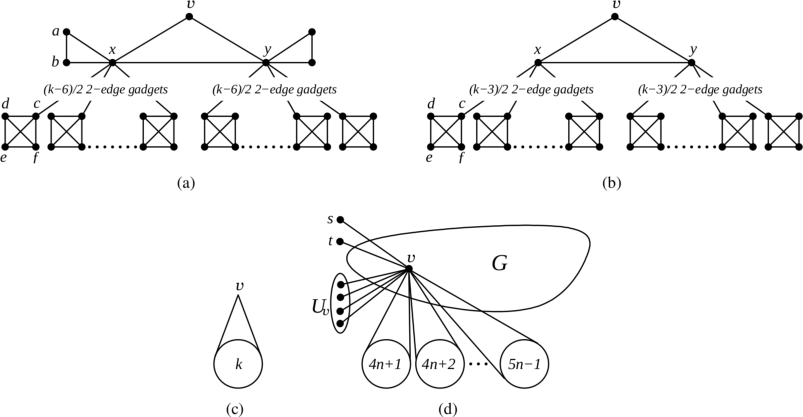
\includegraphics[width=\linewidth]{./images/gadgets}
\caption{}
\label{fig:gadgets}
\end{figure}

Az első ilyen a háromszög-szerkezet. Ez egy olyan $xab$ teljes hármas, melyre külső csúcsból csak $x$-be, a szerkezet tetejébe vezethet él. Figyeljük meg, hogy egy helyes súlyozásban egy ilyen háromszög pontosan $3$-mal járul hozzá az $x$ csúcs összsúlyához. 

A következő a $2$-él-szerkezet, amely egy $cdef$ teljes négyesből és egy erre illeszkedő $xc$ élből áll. Könnyen ellenőrizhető, hogy egy olyan gráf esetében, amely csak az $x$ csúccsal szomszédos, tetszőleges $w$ helyes súlyozásra $w(xc) = 2$. Az $x$ csúcsot a szerkezet végpontjának nevezzük.

Ezek segítségével definiálunk egy harmadik szerkezetet, amelynek $k$-kizáró szerkezet a neve. Itt feltesszük, hogy $k \geq 8$. A szerkezetnek van egy $vxy$ fő háromszöge, ahol a $v$ csúcsot gyökérnek nevezzük. Ezenfelül, ha $k$ páratlan, akkor $x$ és $y$ is $\frac{k - 3}{2}$ diszjunkt $2$-él-szerkezet végpontjai. Amennyiben $k$ páros, úgy $x$ és $y$ is $\frac{k - 6}{2}$ diszjunkt $2$-él-szerkezet végpontjai és egy-egy háromszög-szerkezet tetejei, amelyek szintén diszjunktak. Figyeljük meg, hogy minden $w$ helyes súlyozásban $w(vx) \neq w(vy)$. Ellenkező esetben, mivel a szerkezetek $k - 3$-mal járulnak hozzá $x$ és $y$ összsúlyához, azt kapnánk, hogy $w(x) = w(xv) + w(xy) + k - 3 = w(yv) + w(yy) + k - 3 = w(y)$. Ezért tetszőleges $k$ esetén, ha $w(xy) = 1$, akkor $\lbrace w(x), w(y) \rbrace = \lbrace k - 1, k \rbrace$, illetve ha $w(xy) = 2$, akkor $\lbrace w(x), w(y) \rbrace = \lbrace k, k + 1 \rbrace$. Akárhogy is, $v$-nek van egy $k$ súlyú szomszédja, ezért $w(v) \neq k$. Ezen felül $\lbrace w(vx), w(vy) \rbrace = \lbrace 1, 2 \rbrace$, ezért egy ilyen szerkezet $3$-mal járul hozzá $v$ összsúlyához.

Most már minden eszközünk megvan a redukció elkészítéséhez. Legyen $G = (V, E)$ egy $n$ pontú gráf, ahol feltehetjük, hogy $n \geq 3$. Az $f(G) = (W, F)$ gráfot a következőképpen kapjuk meg $G$-ből. Minden $v \in V$-re
\begin{itemize}
\item összekötjük $v$-t két új csúccsal, $s_v$-vel és $t_v$-vel
\item összekötjük $v$-t egy új $U_v$ halmaz minden csúcsával, ahol $|U_v| = n - 1 - d(v)$
\item felveszünk $n - 1$ új, $v$ gyökerű $k$-kizáró szerkezetet, ahol $k = 4n + 1, 4n + 2, \ldots, 5n - 1$
\end{itemize}

Világos, hogy $f(G)$ polinom időben kiszámítható.

\begin{áll} \label{pro:npreduct}
$f(G)$ bármely $w$ helyes súlyozására az $1, 2$ súlyokkal, $w(v) \in \lbrace 4n - 2, 4n - 1, 4n \rbrace$ minden $v \in V$-re.
\end{áll}

\begin{proof}
Válasszunk egy $v \in V$ csúcsot. Mivel $w(vs_v) + w(vt_v) \in \lbrace 2, 3, 4 \rbrace$, továbbá a $v$ csúcsra $n - 1$ darab $V \cup U_v$-be menő él illeszkedik, és $n - 1$ darab $k$-kizáró szerkezetnek a gyökere, ezért
\begin{equation*}
w(v) \in \lbrace 2, 3, 4 \rbrace + \lbrace n - 1, \ldots, 2n - 2 \rbrace + \lbrace 3n - 3 \rbrace = \lbrace 4n - 2, \ldots, 5n - 1 \rbrace
\end{equation*}
Figyelembe véve, hogy minden $k \in \lbrace 4n + 1, 4n + 2, \ldots, 5n - 1 \rbrace$-re a $v$ csúcs gyökere egy $k$-kizáró szerkezetnek, azt kapjuk, hogy egy $w$ helyes súlyozásban $w(v) \in \lbrace 4n - 2, 4n - 1, 4n \rbrace$.
\end{proof}

Most megmutatjuk, hogy $G \in \textrm{3-SZÍN}$ akkor és csak akkor, ha $f(G) \in \textrm{1-2-SÚLY}$.

Először tegyük fel, hogy $G \in \textrm{3-SZÍN}$. Ez azt jelenti, hogy $G$-nek van egy helyes $3$-színezése. Legyen ez $s: V \rightarrow \lbrace 4n - 2, 4n - 1, 4n \rbrace$. Definiáljunk egy $w: F \rightarrow \lbrace 1, 2 \rbrace$ súlyozást az $f(G)$ gráfon a következő módon. Minden $e \in E$-re legyen $w(e) = 1$. Minden $e = vu$ élre, ahol $v \in V$ és $u \in U_v$, legyen $w(e) = 1$. Minden $v \in V$ csúcsra $s(v) = 4n - 2$ esetén $w(vs_v) = w(vt_v) = 1$, $s(v) = 4n - 1$ esetén $w(vs_v) = 1$ és $w(vt_v) = 2$, valamint $s(v) = 4n$ esetén $w(vs_v) = w(vt_v) = 2$. A szerkezetekhez tartozó éleket az alábbi módon súlyozzuk. Egy $xab$ háromszög-szerkezetre, melynek teteje $x$, legyen $w(xa) = 2$ és $w(xb) = w(ab) = 1$. Egy $xcdef$ $2$-él-szerkezetre, melynek végpontja $x$, legyen $w(xc) = w(cd) = w(ce) = w(de) = w(df) = 2$ és $w(cf) = w(ef) = 1$. Egy $v$ gyökerű és $vxy$ fő háromszögű $k$-kizáró-szerkezet esetén legyen $w(vx) = w(xy) = 2$ és $w(vy) = 1$, minden más él súlyozása pedig a fentieknek megfelelő. Figyeljük meg, hogy $w$ egy helyes színezése $f(G)$-nek, hiszen $w(v) = s(v)$ minden $v \in V$-re.

Tegyük most fel, hogy $G \notin \textrm{3-SZÍN}$. Ennélfogva minden $s: V \rightarrow \lbrace 4n - 2, 4n - 1, 4n \rbrace$-re $s$ nem egy helyes színezés. Ezt összevetve az \ref{pro:npreduct} állítással azt kapjuk, hogy $f(G)$-nek nem létezik helyes súlyozása, azaz $f(G) \notin \textrm{1-2-SÚLY}$.

Ezzel a tételt beláttuk.
\end{proof}

\printbibliography

\end{document}